%\chapter*{Неделя 4}
\protect\thispagestyle{fancy}
\section{}
Предположим, что требуется найти $7$-ой отчет $8$-точечного ДПФ некоторой действительной последовательности. 
Сравнить (заполнить таблицу) количество операций, которое требуется для вычисления $8$-точечного ДПФ по алгоритму БПФ с прореживанием по частоте с числом операций в алгоритме Герцеля.


\begin{center}
	\begin{tabular}{||c|| c | c | c||} 
		\hline
		& БПФ & БПФ ($\mathcal{X}[7]$) & Алгоритм Герцеля ($\mathcal{X}[7]$) \\ [0.5ex] 
		\hline\hline
		\color{teal}{Число действительных сложений и вычитаний} & $14$ & $4$ & $16$ \\ 
		\hline
		\color{orange}{Число действительных умножений} & $0(3)$ & $0(2)$ & $8$ \\
		\hline
		\color{red}{Число комплексных сложений и вычитаний} & $10$ & $3$ & $1$ \\
		\hline
		\color{blue}{Число комплексных умножений} & $5(2)$ & $4(2)$ & $1$ \\
		\hline
	\end{tabular}
\end{center}

Для алгоритма БПФ с прореживанием по частоте найдём общее число операций в графе, которое потребуется, чтобы посчитать весь вектор ДПФ. Также найдём число операций, которое нужно, чтобы найти только один отсчёт $X[7]$. Вo втором случае для наглядности операции выделены в графе соответствующими цветами. Значения в скобках учитывают, что умножение на чисто мнимое число $W^2 = W^2_8 = \exp(-j2\pi\frac{2}{8}) = -j$ в некотором смысле можно считать действительным умножением внутри мнимой части комплексного числа.

\begin{figure}[!h]
	\centering
	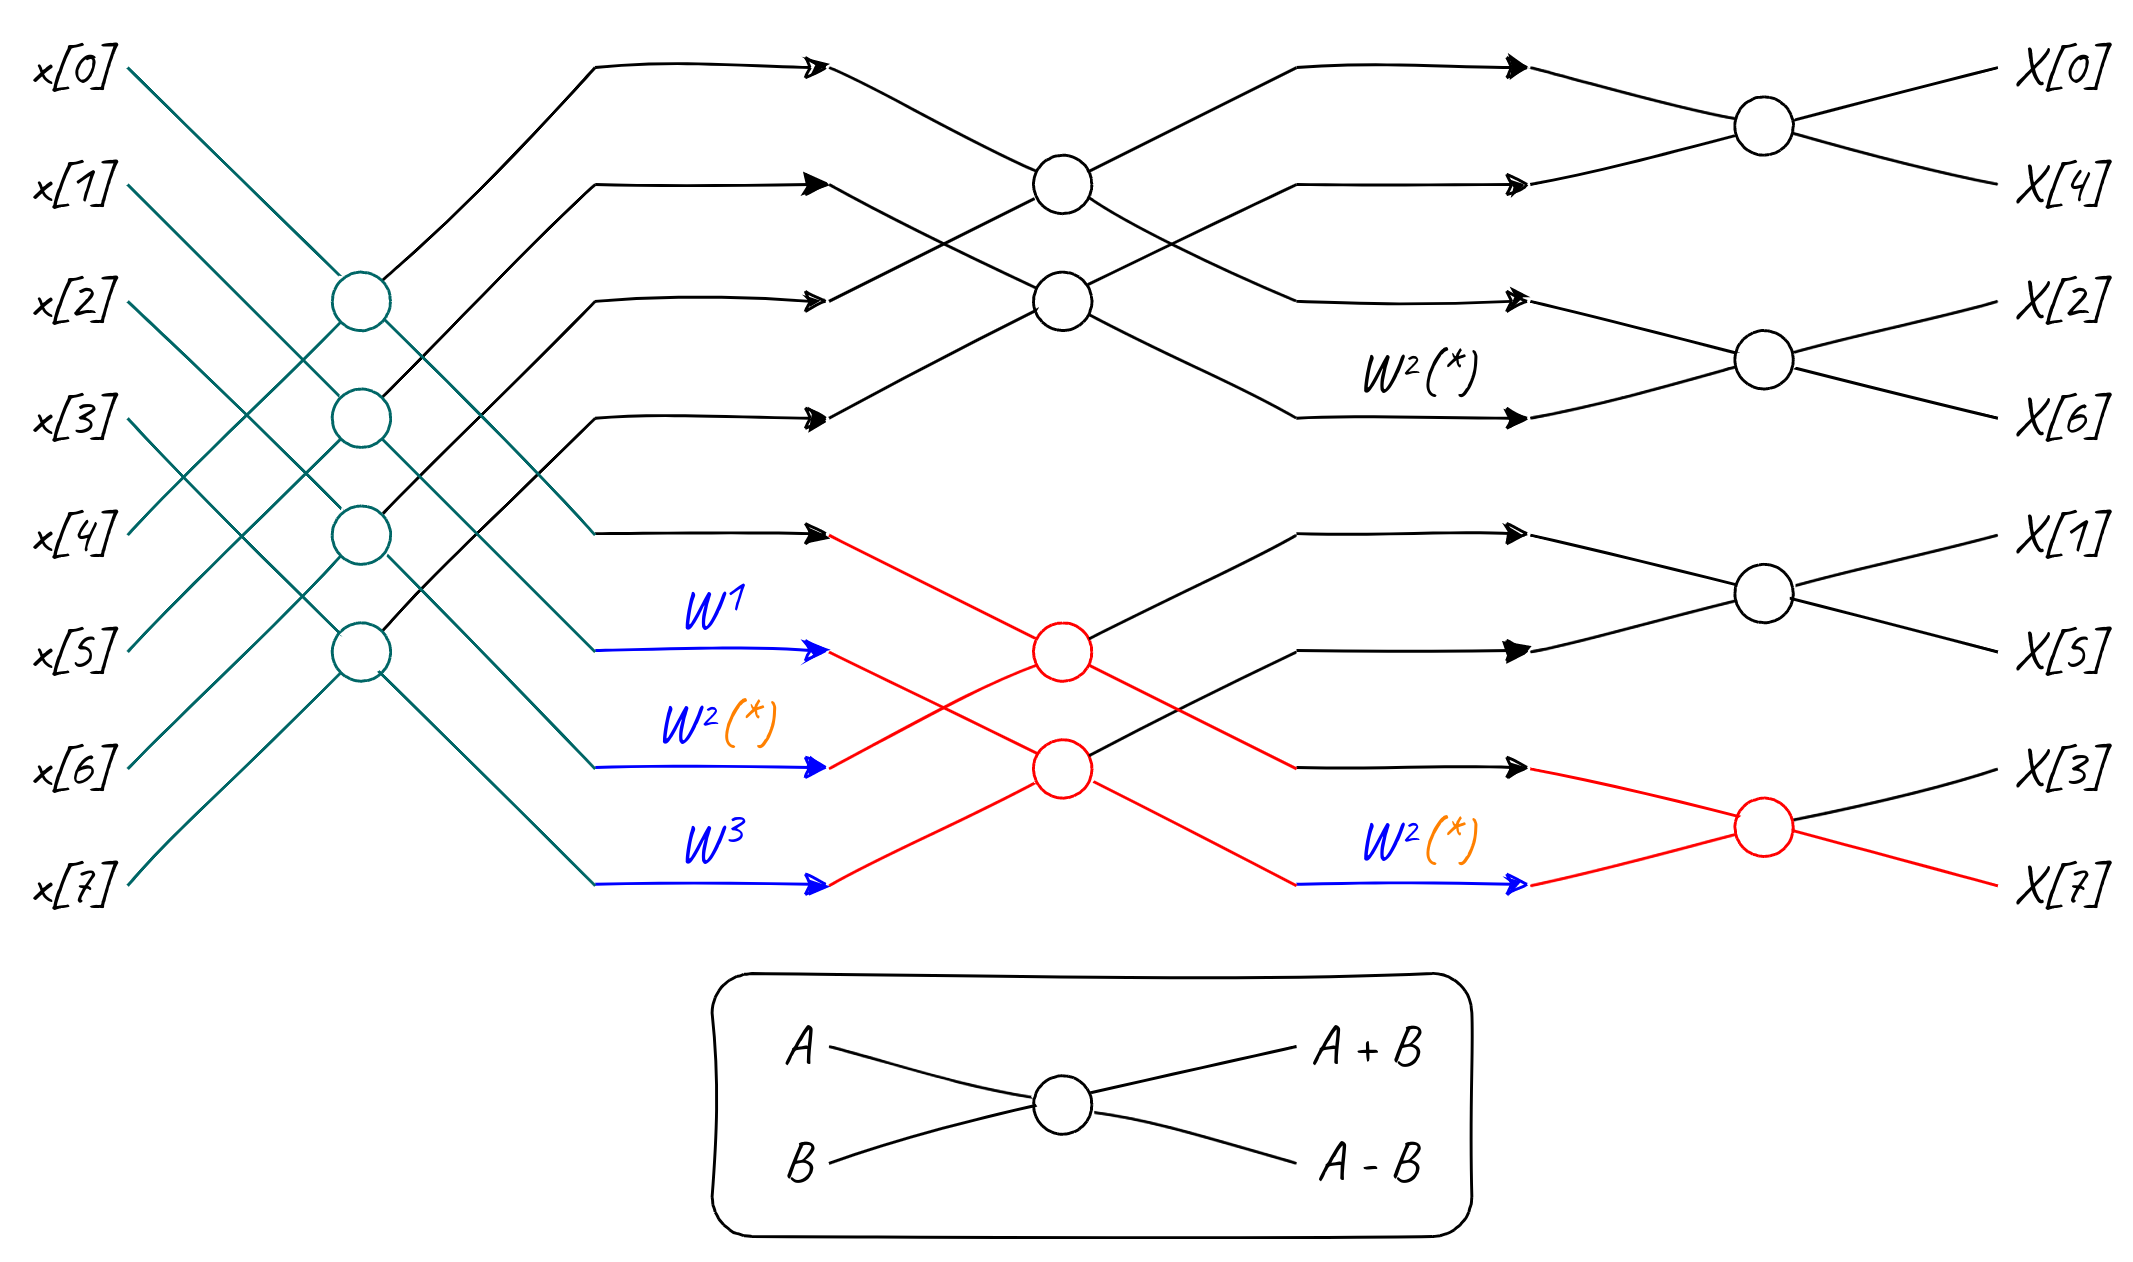
\includegraphics[width=1.\columnwidth]{pics/spring/4/1.png}
	%\caption{.}
	\label{fig:4-1}
\end{figure}

Для поиска $\mathcal{X}[7]$ согласно алгоритму Герцеля будем иметь следующие соотношения. Знаки арифметических операций выделены соответствующими цветами.
\begin{align*}
&\mathcal{V}_7[m] = x[m] \color{teal}+\color{black} 2\cos\left(2\pi \dfrac{7}{8}\right)  \color{orange}\times\color{black} \mathcal{V}_7[m-1] \color{teal}-\color{black} \mathcal{V}_7[m-2],\quad 0\leq m \leq 7,\\
&\mathcal{X}[7] = W^{-7}_8 \color{blue}\times\color{black} V_7[7] \color{red}-\color{black} V_7[6].
\end{align*}


\newpage
\section{}
Пусть требуется вычислить $3$-ий отсчет $64$-точечного ДПФ некоторой действительной последовательности конечной длительности.

Привести блок-схемы фильтров:
\begin{enumerate}[label=(\alph*)]
	\item БИХ-фильтра второго порядка алгоритма Герцеля,
	\item рекурсивного КИХ-фильтра скользящего спектрального анализа.
\end{enumerate}
Указать, как выход фильтра соответствует значению искомого отсчета ДПФ.


\begin{enumerate}[label=(\alph*)]
	\item Схема БИХ-фильтра второго порядка алгоритма Герцеля для поиска $3$-ого отсчета $64$-точечного ДПФ действительной последовательности конечной длительности изображена на рис.~\ref{fig:4-2-1}. При этом правую часть фильтра (в красной рамке) достаточно вычислить лишь один раз на финальном этапе. Искомый отсчёт ДПФ будет равен выходу фильтра (с правой частью) на последней $63$-ей итерации (считая с нулевой).
	
	\begin{figure}[!h]
		\centering
		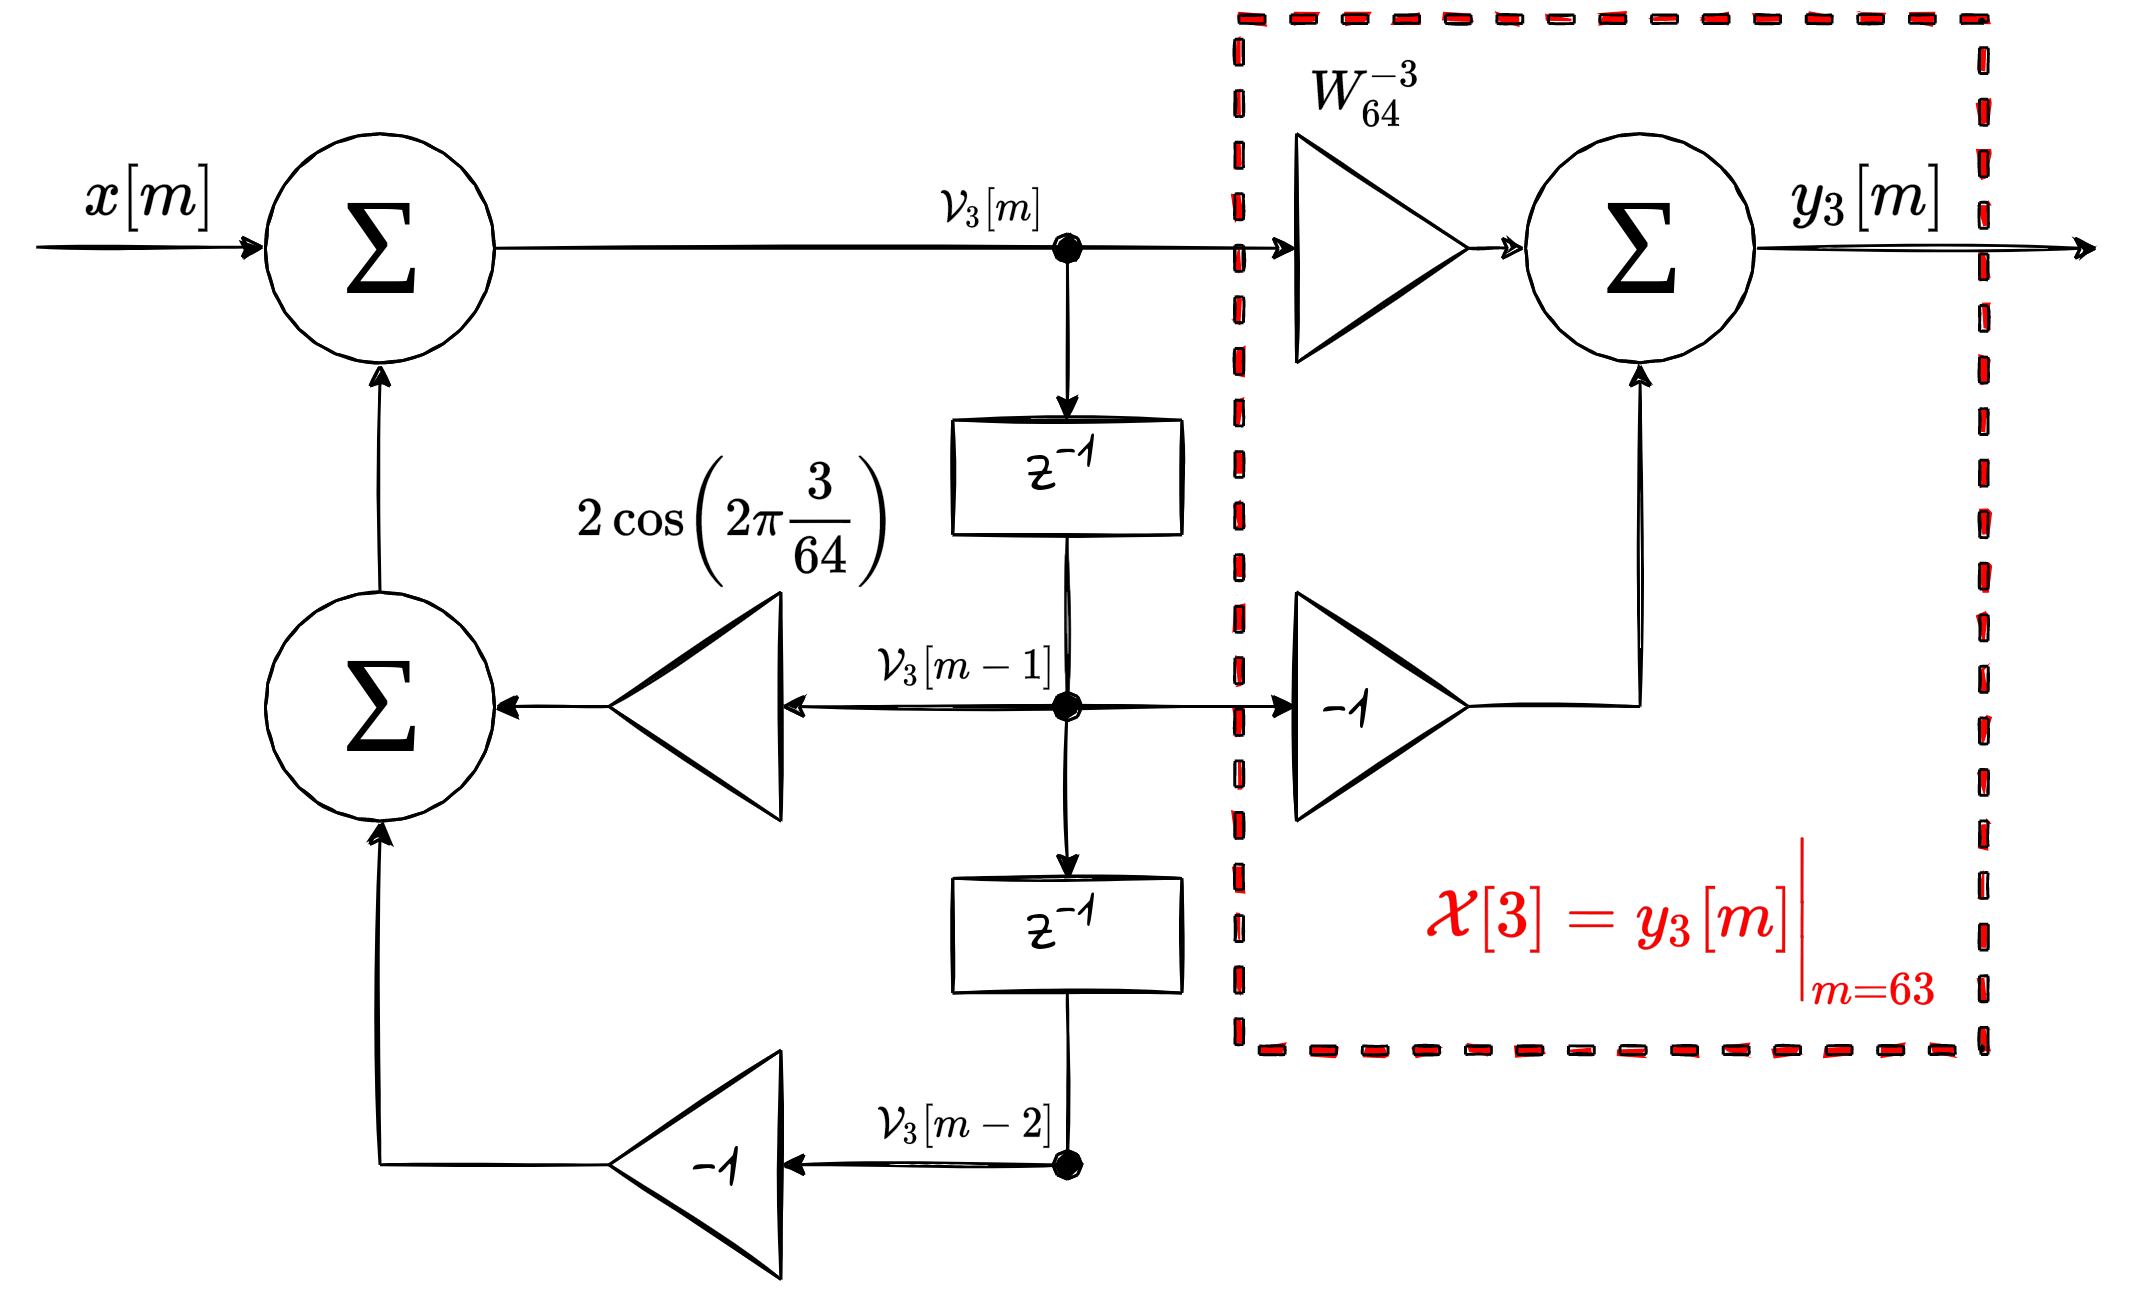
\includegraphics[width=0.65\columnwidth]{pics/spring/4/2-1.png}
		\caption{Схема БИХ-фильтра второго порядка алгоритма Герцеля.}
		\label{fig:4-2-1}
	\end{figure}
	
	
	\item На рис.~\ref{fig:4-2-2} представлена схема рекурсивного КИХ-фильтра скользящего однобинового спектрального анализа для поиска $3$-ого отсчета $64$-точечного ДПФ действительной последовательности конечной длительности.
	Искомый отсчёт ДПФ будет равен выходу фильтра на $63$-ей итерации алгоритма (считая с нулевой).
	\begin{figure}[!h]
		\centering
		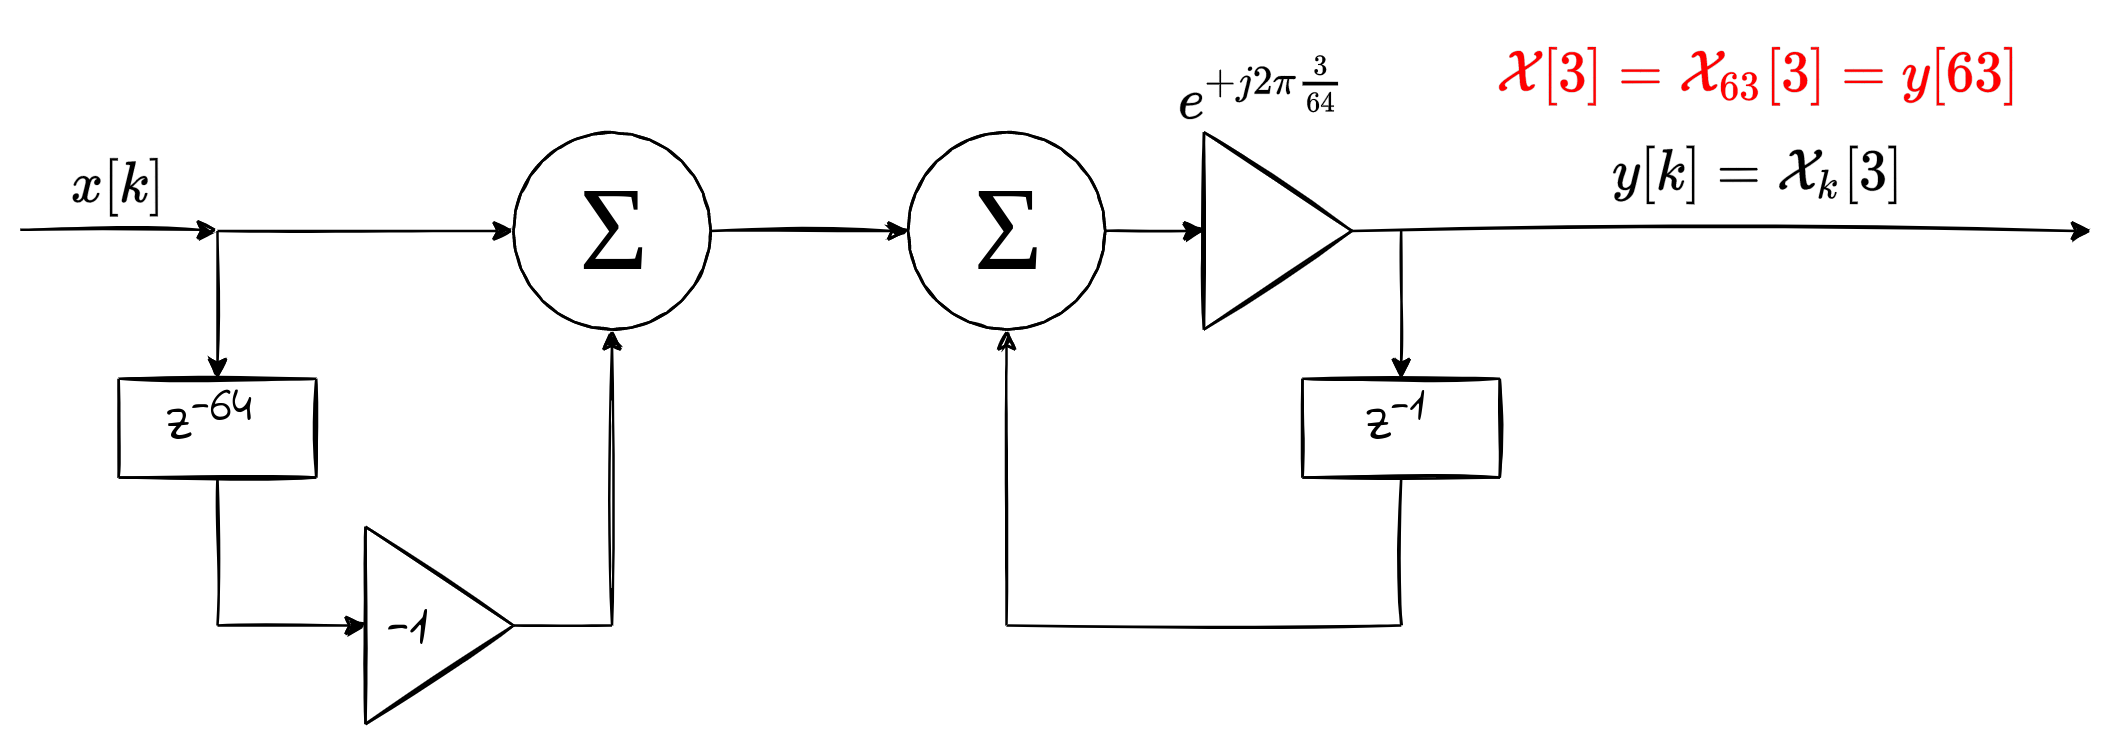
\includegraphics[width=0.65\columnwidth]{pics/spring/4/2-2.png}
		\caption{Схема рекурсивного КИХ-фильтра скользящего однобинового спектрального анализа.}
		\label{fig:4-2-2}
	\end{figure}
	
\end{enumerate}


\newpage
\section{}
Предположим, что с помощью окна длиной $M = 4000$ осуществляется вычисление кратковременного дискретного преобразования Фурье последовательности

\begin{equation*}
x[k] = \cos\left(2\pi\dfrac{f_1}{f_d}k + \varphi_1\right) +
\cos\left(2\pi\dfrac{f_2}{f_d}k + \varphi_2\right)
\end{equation*}

длиной в $N = 40000$ отсчетов без перекрытия. Фазы $\varphi_1$ и $\varphi_2$ неизвестны. Частота дискретизации $f_d = 44100 $ Hz.

Для случая окна Ханна указать, начиная с какого значения $\Delta f = |f_1 - f_2|$ можно выбором необходимой размерности ДПФ $N_{\text{FFT}}$ обеспечить различимость гармонических компонент на спектрограмме.

Спектральные компоненты будут гарантировано различимы, если $\Delta f = |f_1 - f_2| \geq \Delta f_{-6\text{dB}}$.

\begin{equation*}
\Delta f = |f_1 - f_2| \geq \Delta f_{-6\text{dB}} = f_d \cdot \max \left\{\Delta \nu_{-6\text{dB}}, \dfrac{2}{N_{\text{FFT}}}\right\} =
f_d \cdot \max\left\{\dfrac{2.0}{M}, \dfrac{2}{N_{\text{FFT}}}\right\} = \dfrac{2f_d}{M} = 22.05\text{ Hz}.
\end{equation*}
